\documentclass[../BTL.tex]{subfiles}
\begin{document}
\section{Phân tích thiết kế CSDL}
Từ mô tả bài toán, nhóm tiến hành vẽ lược đồ quan hệ của BTL được mô tả như trên hình \ref{fig:relation-schema}. Từ lược đồ này, áp dụng các quy tắc chuyển từ lược đồ quan hệ sang các bảng của cơ sở dữ liệu, ta được biểu đồ E-R của cơ sở dữ liệu như trên hình \ref{fig:EER}. Cụ thể như sau:

\subsection{Các thực thể chính:}
\begin{itemize}
    \item Club: Thông tin về câu lạc bộ (tên, quốc gia, sân vận động)
    \item HeadCoach: Thông tin về huấn luyện viên (tên, ngày sinh, quốc tịch)
    \item Player: Thông tin về cầu thủ (tên, ngày sinh, số áo, vị trí)
    \item League: Thông tin về giải đấu
    \item LeagueSeason: Mùa giải của một giải đấu
    \item Match: Thông tin trận đấu giữa các câu lạc bộ
    \item MatchAction: Hành động trong trận đấu (bàn thắng, thẻ, kiến tạo)
    \item ClubSeasonTable: Bảng xếp hạng của câu lạc bộ trong một mùa giải
\end{itemize}
\subsection{Các quan hệ chính:}
\begin{itemize}
    \item Club - ClubSeasonTable: 1-n (một câu lạc bộ có nhiều bảng xếp hạng qua các mùa)
    \item Club - Match: 1-n (một câu lạc bộ có thể tham gia nhiều trận với vai trò chủ nhà/khách)
    \item HeadCoach - CoachClub: 1-n (một HLV có thể dẫn dắt nhiều CLB qua thời gian)
    \item League - LeagueSeason: 1-n (một giải đấu có nhiều mùa giải)
    \item LeagueSeason - ClubSeasonTable: 1-n (một mùa giải có nhiều bảng xếp hạng của các CLB)
    \item Match - MatchAction: 1-n (một trận đấu có nhiều hành động)
    \item Player - MatchAction: 1-n (một cầu thủ thực hiện nhiều hành động trong trận)
\end{itemize}
\begin{figure}
    \centering
    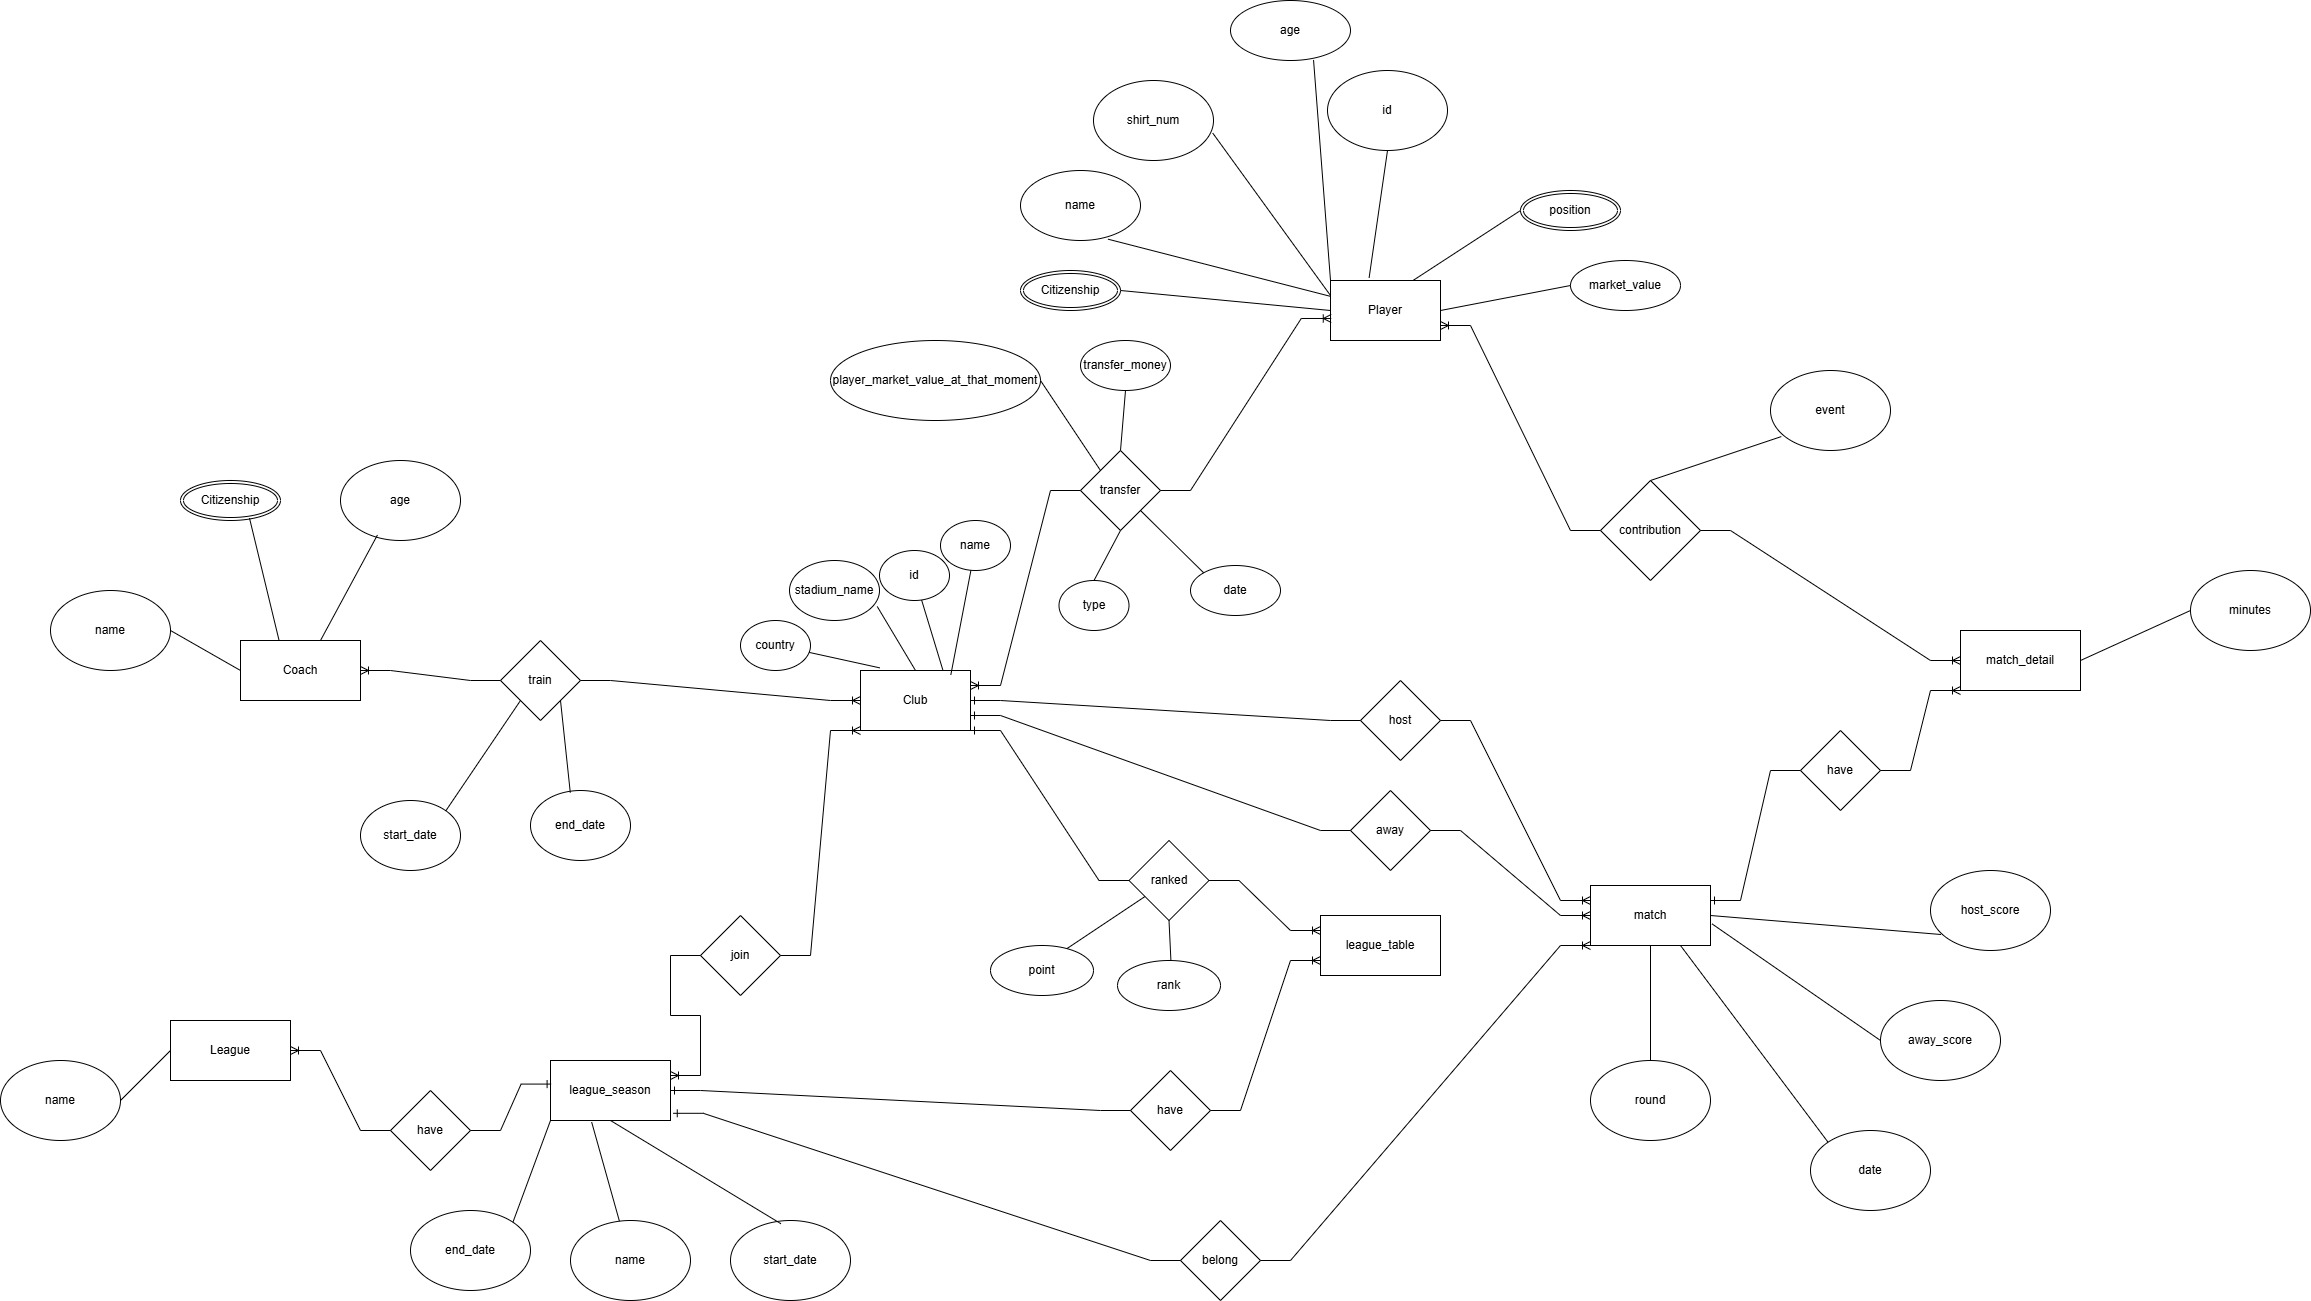
\includegraphics[width=1\linewidth]{Hinhve/relation-schema.jpg}
    \caption{Lược đồ quan hệ}
    \label{fig:relation-schema}
\end{figure}

\begin{figure}
    \centering
    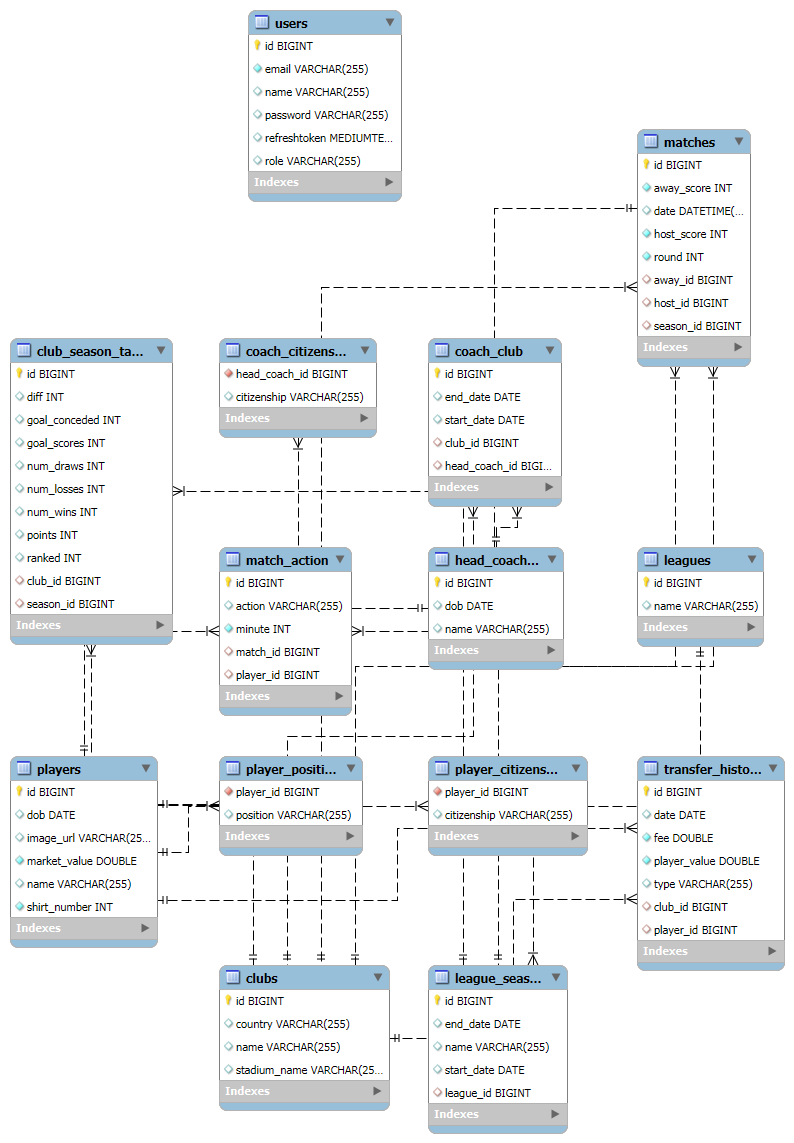
\includegraphics[width=1\linewidth]{Hinhve/EER.png}
    \caption{Biểu đồ E-R của cơ sở dữ liệu}
    \label{fig:EER}
\end{figure}
\section{Phân tích thiết kế chức năng}
\subsection{Kiến trúc tổng thể:}
Hệ thống website thống kê bóng đá được xây dựng theo kiến trúc phân lớp Client-Server với mô hình Single Page Application (SPA) ở phía frontend \cite{react-docs} \cite{antd-docs} và RESTful API ở phía backend\cite{hoidanit-restful} \cite{vanthoi-github}. Lược đồ mô tả kiến trúc của hệ thống như trên hình \ref{fig:web-overall-architecture}. Frontend được xây dựng dựa trên React và Vite với kiến trúc dựa trên thành phần(component-based), tối ưu cho việc phát triển và bảo trì. Backend được thiết kế theo cấu trúc RESTful API, với các điểm cuối(endpoint) hay URL cung cấp dữ liệu cho frontend. Hệ thống sử dụng cơ chế JWT để xác thực người dùng: 
\begin{itemize}
    \item Đăng nhập: User cung cấp email/password, server trả về access token
    \item Xác thực API: Token được gửi trong Authorization header trong Http request
    \item Phân quyền: Phân biệt user thường và admin để hạn chế quyền truy cập và sử dụng thành phần <PrivateRoute>  kiểm tra token hợp lệ trước khi vẽ giao diện cho admin
\end{itemize}


\begin{figure}
    \centering
    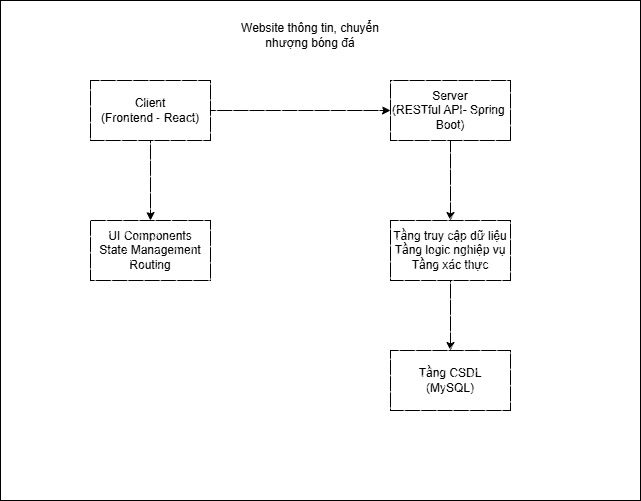
\includegraphics[width=1\linewidth]{Hinhve/web-overall-architecture.jpg}
    \caption{Lược đồ mô tả kiến trúc của hệ thống}
    \label{fig:web-overall-architecture}
\end{figure}


\subsection{Các module chức năng chính:}
\subsubsection{Quản lý người dùng}
\begin{itemize}
    \item Đăng nhập/Đăng ký: Cho phép người dùng tạo tài khoản và đăng nhập
    \item Phân quyền: Phân biệt người dùng thông thường và admin
    \item Quản lý session: Sử dụng token để xác thực API
\end{itemize}
\subsubsection{Quản lý cầu thủ:}
\begin{itemize}
    \item Xem danh sách cầu thủ: Hiển thị danh sách cầu thủ có phân trang
    \item Tìm kiếm và lọc: Cho phép tìm kiếm theo tên và lọc theo vị trí, quốc tịch, CLB
    \item Chi tiết cầu thủ: Hiển thị thông tin chi tiết, lịch sử chuyển nhượng
    \item Thêm/sửa/xóa cầu thủ (chỉ admin)
\end{itemize}
\subsubsection{Quản lý câu lạc bộ:}
\begin{itemize}
    \item Xem danh sách CLB: Hiển thị danh sách CLB có phân trang
    \item Tìm kiếm và lọc: Cho phép tìm kiếm theo tên và lọc theo quốc gia
    \item Chi tiết CLB: Hiển thị thông tin chi tiết, đội hình, lịch sử chuyển nhượng
    \item Thống kê CLB: Cầu thủ ghi nhiều bàn thắng, kiến tạo nhiều nhất
    \item Thêm/sửa/xóa CLB (chỉ admin)
\end{itemize}
\subsubsection{Quản lý huấn luyện viên:}
\begin{itemize}
    \item Xem danh sách HLV: Hiển thị danh sách HLV có phân trang
    \item Tìm kiếm và lọc: Cho phép tìm kiếm theo tên và lọc theo quốc tịch, CLB
    \item Chi tiết HLV: Hiển thị thông tin chi tiết, lịch sử làm việc
    \item Thêm/sửa/xóa HLV (chỉ admin)
\end{itemize}
\subsubsection{ Quản lý giải đấu(chỉ admin):}
\begin{itemize}
    \item Xem danh sách giải đấu: Hiển thị các giải đấu
    \item Chi tiết giải đấu: Hiển thị thông tin chi tiết, các mùa giải
    \item Thêm/sửa/xóa giải đấu (chỉ admin)
\end{itemize}
\subsubsection{Quản lý mùa giải(chỉ admin):}
\begin{itemize}
    \item Thêm/sửa/xóa mùa giải: Quản lý các mùa giải của một giải đấu
    \item Quản lý CLB trong mùa giải: Thêm CLB, cập nhật thành tích (thắng, hòa, thua)
    \item Quản lý trận đấu: Lịch thi đấu, kết quả, sự kiện trong trận
\end{itemize}
\subsubsection{Thống kê và phân tích:}
\begin{itemize}
    \item Bảng xếp hạng: Hiển thị BXH của mùa giải
    \item Top ghi bàn: Cầu thủ ghi nhiều bàn nhất
    \item Top kiến tạo: Cầu thủ kiến tạo nhiều nhất
    \item Thẻ phạt: Thống kê thẻ vàng, thẻ đỏ
    \item Tự động cập nhật bảng xếp hạng sau khi cập nhật kết quả trận đấu
    \item Tính toán thống kê số trận thắng, hòa, thua và điểm số
\end{itemize}
\subsubsection{Tương tác giao diện:}
\begin{itemize}
    \item Responsive design: Hỗ trợ nhiều kích thước màn hình
    \item Tìm kiếm nâng cao: Cho phép tìm kiếm theo nhiều tiêu chí
    \item Hiển thị danh sách: Sử dụng Table component của Ant Design với phân trang, sắp xếp
    \item Forms: Form thêm/sửa với kiểm tra đầu vào
\end{itemize}
\subsubsection{Xử lý nghiệp vụ đặc biệt:}
\begin{itemize}
    \item Tự động cập nhật bảng xếp hạng sau khi thêm/sửa/xóa trận đấu
    \item Tính toán lại điểm, bàn thắng, bàn thua khi cập nhật kết quả
    \item Tìm HLV/CLB hiện tại dựa trên ngày bắt đầu/kết thúc hợp đồng
\end{itemize}
\section{Các chức năng chưa làm được}
\subsection{Sửa đổi thông tin cá nhân tài khoản}
Do thời gian có hạn và phải tập trung vào những tính năng quan trọng khác liên quan đến giải đấu, bảng xếp hạng nên nhóm em chưa thể thực hiện phần chức năng này

\subsection{ Tự động lấy dữ liệu từ những trang web cung cấp dữ liệu}
Đây là một việc tương đối khó khi phải cập nhật dữ liệu trận đấu, chuyển nhượng mới nhất từ trên những trang thông tin bóng đá do phải thực hiện việc cào và xử lý dữ liệu. Nên phần này sẽ được đưa vào hướng phát triển tiếp theo của BTL

\subsection{ Những thống kê phức tạp hơn liên quan đến cầu thủ}
Ví dụ như số trận ghi bàn liên tiếp, số trận thắng liên tiếp trong một mùa giải của câu lạc bộ,phân tích đối đầu giữa các đội, thống kê chi tiết trong trận đấu - tỷ lệ kiểm soát bóng, số cú sút trúng đích,.. Đây đều là những thống kê phức tạp và đòi hỏi những câu lệnh truy vấn phức tạp và cũng sẽ được đưa vào hướng phát triển tiếp theo của BTL

\subsection{ Báo cáo và xuất dữ liệu}
Một chức năng khác khá hữu ích là báo cáo và xuất dữ liệu, đây cũng là một chức năng mà nhóm chưa làm được và sẽ được đưa vào hướng phát triển của nhóm

\subsection{ Tối ưu hóa hệ thống}
Do chưa có kiến thức cũng như chưa thực hành nhiều nên nhóm em chưa thể áp dụng những kiến thức về thiết kế hệ thống và tối ưu hóa hệ thống được. Do đó đây cũng là phần nhóm em muốn thêm vào phần hướng phát triển
\end{document}